\documentclass[svgnames,tikz]{standalone}
\usepackage{pgfmath}
\usetikzlibrary{positioning,arrows,calc,3d}

\tikzset{
  focus/.style args={#1 at #2}{
    insert path={
      %{ [white] (#2.north east) rectangle (#2.south west)}
      ($(#2.center)!#1!(#2.north east) $) rectangle ($(#2.center)!#1!(#2.south west) $)
    }
  },
  focusout/.style args={#1 at #2}{
    even odd rule,
    insert path={
      (#2.north east) rectangle (#2.south west)
      ($(#2.center)!#1!(#2.north east) $) rectangle ($(#2.center)!#1!(#2.south west) $)
    }
  },
  txt/.style={font=\Large\tt},
  img/.style={
     inner sep=2pt,
     draw,
     label/.append style={font=\small\tt},
  },
}


\begin{document}
\begin{tikzpicture}
\tikzset{every node/.style={node distance=5pt, font=\Huge}}

\node[txt] (p0) { green( };

\node[img, yslant=.5] (p1) [right=0.9cm of p0.center] { 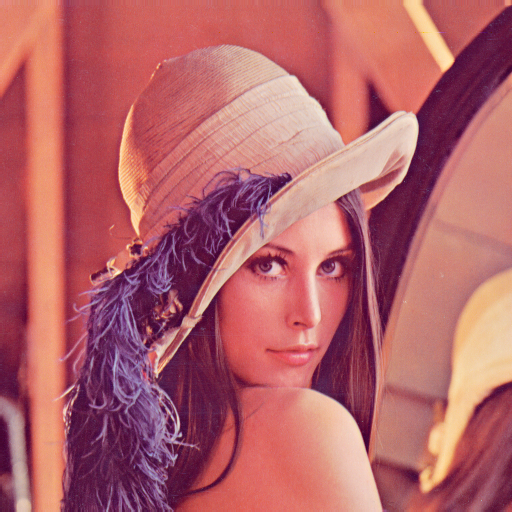
\includegraphics[width=3cm]{../../images/lena_color.png}};

\node[txt] (p2) [right=4.1cm of p0.center] { ) $\rightarrow$ };

\node[img, yslant=.5] (p3) [right=5.6cm of p0.center] { 
\includegraphics[width=3cm]{../../images/lena_green.png}};

\end{tikzpicture}
\end{document}